\chapter{Analyzing Classes}
Python has two different kinds of classes, namely new and old style (or classic) classes that both supports multiple inheritance (note that from Python 3 all classes are new style classes). A new style class is one that contrary to an old style class is a subclass of \inlinecode{object}. The two different kinds of classes vary among others in their method resolution order (MRO)\cite{pyref.typehierarchy}: old style classes resolves variables and attributes by a depth-first, left-to-right strategy, whereas new style classes uses the more complex strategy C3\cite{pyref.c3mro}, which is also known as the call-next-method from other multiple inheritance languages. Also, the built in function \inlinecode{super} can only be used with new style classes. In this section we present our work towards handling those two kinds of classes.

To start with consider the below example that illustrates the difference in MRO between new and old style classes.

\begin{listing}[H]
	\begin{minted}[linenos]{python}
class A():
	x = 'A'
class B(A): pass
class C(A):
	x = 'C'
class D(B, C): pass
D().x # 'A'
	\end{minted}
	\caption{Multiple inheritance}\label{code:OldStyleMROExample}
\end{listing}

Since \inlinecode{D} extends \inlinecode{B} and \inlinecode{C}, which in turn extends the old style class \inlinecode{A}, \inlinecode{D} is itself an old style class. Therefore, evaluating \inlinecode{D().x} will result in \inlinecode{'A'}. If we instead had declared \inlinecode{A} as a new style class \inlinecode{class A(object): ...}, evaluating \inlinecode{D().x} would result in \inlinecode{'C'}.


\subsection{Class declarations}
To start with we must take care of class declarations. In the CFG we have the following nodes related to this: \textit{ClassDeclNode}, \textit{ClassEntryNode}, and \textit{ClassExitNode}. Consider a class declaration like \inlinecode{class C(B1,...,Bn):<body>}. For this particular code we create a class declaration node in our CFG which holds the name of the class and the names of the baseclasses, i.e. \inlinecode{C}, and \inlinecode{B1}, ..., \inlinecode{Bn}. Furthermore we create a class entry node which we make the successor of the class declaration node. Then the inductively created CFG for the piece of code appearing at \inlinecode{<body>} will be inserted after the class entry node, and finally, we create a class exit node and make it the successor of the exit node of the inductively created \inlinecode{<body>} CFG.

More or less, the purpose of the three different kinds of nodes is the following:

\begin{itemize}
	\item The class declaration node, \textit{ClassDeclNode}, creates one or more class objects on the heap and writes the variable \inlinecode{C} as a property on each object that is on top of on of the scope chains.
	\item The class entry node, \textit{ClassEntryNode}, modifies the set of execution contexts by pushing the newly created class object on top of each of them.
	\item The class exit node, \textit{ClassExitNode}, reverts the execution contexts to what they were before visiting the class entry node (by popping the newly created class object from each of the execution contexts).
\end{itemize}

\subsubsection{Creating the class objects on the heap}
As mentioned our type analysis creates one or more class object on the heap whenever a class declaration node is meet. More precisely:

\begin{itemize}
	\item If \inlinecode{C} is definately a new style class a new style class object is created on the heap. Likewise for old style classes.
	\item Otherwise, both a new style class object and an old style class object is created on the heap.
\end{itemize}

For the example in listing \ref{code:OldStyleMROExample} our analysis will only create an old style class object on the heap, however for the below example we generate two objects.

\begin{listing}[H]
	\begin{minted}[linenos]{python}
if (...):
	class B(): pass
else:
	class B(object): pass
class C(B): pass
	\end{minted}
	\caption{An example where we can't conclude that \inlinecode{C} is definately a new style class or definately an old style class.}\label{code:NotDefinatelyNewOldStyleClass}
\end{listing}

We conclude that a class is definately a new style class if the following holds:

\begin{enumerate}
	\item The built in class \inlinecode{object} has not been overwritten.
\end{enumerate}

Of course it would still be possible to conclude that \inlinecode{class C(O): ...} is a new style class if the variable \inlinecode{O} has been set to \inlinecode{object} before overwriting \inlinecode{object} like in the below example.

\begin{listing}[H]
	\begin{minted}[linenos]{python}
O = object
object = 42
class C(O): pass
	\end{minted}
	\caption{The class \inlinecode{C} here is easily seen to be a new style class.}\label{code:ClassOverwrittenObject}
\end{listing}

However, our implementation does not at the moment check this because of the limited time of our project, and the fact that programmers should really not overwrite the built in \inlinecode{object}. Note that our implementation does conclude that \inlinecode{class C(O): ...} is a new style class if line 2 in the example had been skipped.

If \inlinecode{object} has not been overwritten, we check that:

\begin{enumerate}
\setcounter{enumi}{1}
	\item All the base classes \inlinecode{B1}, ..., \inlinecode{Bn} are either the built in object or definately a new style class.
\end{enumerate}

Recall that the baseclasses \inlinecode{B1}, ..., \inlinecode{Bn} are just variablenames. If \inlinecode{Bi} is the variable \inlinecode{object}, we can conclude that it is the built in object since we from (1) have that the built in \inlinecode{object} has not been overwritten. If \inlinecode{Bi} is not \inlinecode{object} we look up the variable on the scope chain, and make sure its value is only a pointer to a new style class object on the heap, or the built in class \inlinecode{object}. If it is for instance a pointer to either a new style class object or an old style class object (see for instance listing \ref{code:NotDefinatelyNewOldStyleClass}), we conclude that the class \inlinecode{C} it is not definately a new style class object.

In the same way we conclude that a class is definately an old style class.

\subsubsection{Populating the class objects on the heap with fields and methods}
As mentioned above the heap objects we create at class declaration nodes are empty. We add fields and methods to these heap objects inbetween the class entry and class exit nodes. First, let us investigate how fields and methods are created for classes below.

Fields and methods can be created at class declaration time, and dynamically added to the class after declaration as the following tries to illustrate:

\begin{listing}[H]
	\begin{minted}[linenos]{python}
class C(object):
	x = 10
	def getX(self):
		return self.x
def setX(self, x):
	self.x = x
C.setX = setX
	\end{minted}
	\caption{Adding a field \inlinecode{x} and methods \inlinecode{getX} and \inlinecode{setX} on a class.}\label{code:FieldAndMethodOnClass}
\end{listing}

We can handle this quite easily in our analysis by just updating the scope chains at class entry: we push the relevant class object on the heap (whether it is a new or an old style class) onto each current scope chain. As a result when we write to a variable like \inlinecode{x} inside the class it will be written to the head of each scope chain, i.e. the class heap object, which is exactly what we want.

This is however not quite enough in order to support methods since our CFG does not distinguish between function and method declarations. Thus \inlinecode{getX} will appear as a function declaration in our CFG, even though it is actually a method. We handle this at function declaration time by checking whether the head of the scope chain is a class object. In that case we wrap the function in an unbound method object, which is merely just a pointer to the function object. Otherwise we proceed as we would otherwise have handled a function declaration as explained in section TODO\todo{Fix section}.

We wrap the function in an unbound method object for at least two reasons:

\begin{enumerate}
	\item It is not possible to write properties on methods, but properties on methods can be read in case the underlying function has the property.
\end{enumerate}

This is illustrated by the following example:

\begin{listing}[H]
	\begin{minted}[linenos]{python}
class C(object): pass

def foo(self): pass
foo.prop = 42

C.foo = foo
C.foo.prop # 42
C.foo.prop = 0 # AttributeError
	\end{minted}
	\caption{It is not possible to set properties on methods.}\label{code:FieldAndMethodOnClass}
\end{listing}

\begin{enumerate}
\setcounter{enumi}{1}
	\item When creating a class instance the unbound methods of the class are turned into bound methods on the instance object (we concentrate on this in the following section, Handling object creations\todo{Add ref to section?}).
\end{enumerate}

Fields and methods can also be added to a class after declaration time as was illustrated in example \ref{code:FieldAndMethodOnClass}. In our CFG this is represented by a \textit{WriteVariableNode}, so what we do in this case is very simular to what we do inbetween the class entry and exit nodes: if the object being written to is a class object, and the value being written is a function, then we wrap it in an unbound method object. Otherwise we just write the value to the property of the object as we would normally have done.


\subsection{Handling object creations}
When an instance of a class is created each unbound method of the class is turned into a bound method on the object. The purpose of the bound method is to pass the instance reference as the first argument to the unbound method (the \inlinecode{self} argument). As a consequence our lattice, unlike e.g. the lattice used by the TAJS Analyzer, does not contain an explicit representation of the \inlinecode{this} object (it is simply treated as a normal parameter to the function). The below example illustrates the implicit passing of the self parameter for bound methods:

\begin{listing}[H]
	\begin{minted}[linenos]{python}
class C(object):
	def foo(self):
		pass

C.foo # <unbound method C.foo>

x = C()
x.foo # <bound method C.foo of <C object at ...>>

x.foo() # self implicitly passed as self
C.foo(x) # using the unbound method by explicitly passing an instance

# TypeError: unbound method foo() must be called with C instance as 
# first argument (got nothing instead)
C.foo()
	\end{minted}
	\caption{Bound and unbound methods.}\label{code:BoundAndUnboundMethodsOnClass}
\end{listing}

Contrary to e.g. JavaScript, class instances are not created using the \inlinecode{new} keyword as can be seen from the above example. This means that we can't necessarily distinguish a function call from an object creation.

At each function call (i.e. \textit{ClassNode} in our CFG) we therefore investigate which kind of object label on the heap we are calling\footnote{It is of course a \inlinecode{TypeError} whenever the value being called is something that is not only a function object, a function wrapper object, a class object, or a method object}. If we happen to call a new style class object on the heap, we create a new style instance object on the heap, representing the newly created instance (likewise for old style classes). In particular, we do not modify the call graph as we do for function calls unless the magic method \inlinecode{\_\_init\_\_} has been implemented on the class (see the following section, Supporting constructor calls\todo{Insert reference to section}, on how we handle this).

Of course we wish generate the class instance objects conservatively. Consider the following code:

\begin{listing}[H]
	\begin{minted}[linenos]{python}
if (...):
	class C(): pass
elif (...):
	class C(object): pass
else:
	def C():
		return 42
x = C()
	\end{minted}
	\caption{Difference between methods and functions on classes.}\label{code:BothNewOldClassAndFunction}
\end{listing}

For this code we can't tell whether \inlinecode{C} after the \inlinecode{if} statement is the old style class in line 2, the new style class in line 4 or the function in line 6. Therefore, our analysis will conclude that \inlinecode{x} is either a pointer to a new style class instance, a pointer to an old style class instance, or the integer 42. This is seen in the figure below generated by our type analysis, which is the output of the heap at the exit node of the CFG of the code in example \ref{code:BothNewOldClassAndFunction}.

\begin{listing}[H]
	\begin{center}
		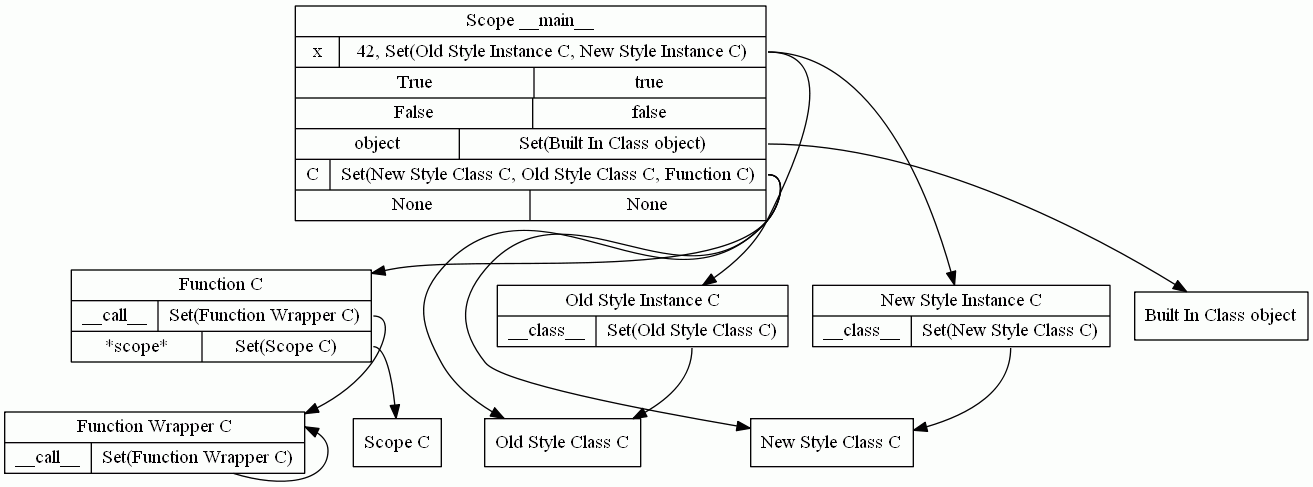
\includegraphics[width=1\textwidth]{images/BothNewOldClassAndFunction.png}
	\end{center}
	\vspace{-10pt}
	\caption{The heap generated by our analysis tool.}
	\label{fig:BothNewOldClassAndFunction}
\end{listing}

So far we haven't mentioned how we populate the newly created class instance object with the fields of the class, but this is more or less trivial: Each field (i.e. attribute) of the class is copied to the instance object, and each unbound method of the class is transformed into a bound method on the instance object (i.e. we create a new bound method object on the heap for each unbound method on the class).


\subsection{Supporting constructor calls}
The magic method \inlinecode{\_\_init\_\_} can be set on a class in order to supply a constructor as the following illustrates:

\begin{listing}[H]
	\begin{minted}[linenos]{python}
class C(object):
	def __init__(self, x):
		self.x = x

c = C(42)
c.x # 42
	\end{minted}
	\caption{The \inlinecode{\_\_init\_\_} magic method.}\label{code:InitConstructorClass}
\end{listing}

This introduces a minor issue that arises from the fact that we cannot at first sight distinguish between object creations and usual function calls (recall that Python has no \inlinecode{new} keyword). What happens at line 5 in example \ref{code:InitConstructorClass} above is the following:

\begin{enumerate}
	\item A new style instance object is created on the heap because of the call to a new style class object.
	\item A value pointing to this newly created instance object is stored in the special return register on the stack.
	\item The call graph is updated with call edges from the call node to the entry node of \inlinecode{\_\_init\_\_}, and from the exit node of \inlinecode{\_\_init\_\_} to the after call node.
	\item As a result of (3), the return value of \inlinecode{\_\_init\_\_} is stored in the special return register. Note that the return value of \inlinecode{\_\_init\_\_} must be the built in constant \inlinecode{None}; otherwise a type error results (for this example our CFG will insert an implicit return \inlinecode{None} node).
	\item The after call node will now read the value from the special return register on the stack and store it; in this case as the attribute \inlinecode{x} of \inlinecode{c}.
\end{enumerate}

For this approach the best we can do is to take the least upper bound when we write to the special return register. As a consequence the variable \inlinecode{c} from the example will after the object creation be set to the value corresponding to either being \inlinecode{None} or a new style instance object (meaning that we should report a type error in line 6, because a property is possibly being dereferenced on a non-object!).

We solve this issue by introducing a new special constructor return register, where we store newly created class instances in, together with a new kind of call edge in the call graph; constructor call edges.

The idea is the following: Instead of updating the call graph with call edges in (3), we update it with constructor call edges. This means that we can recognize returns from \inlinecode{\_\_init\_\_} functions, check that they are indeed \inlinecode{\_\_None\_\_} (otherwise raise a type error) and then ignore it.

Specifically, our implementation has a special join operation for after call nodes (for all other nodes the join operation just takes the least upper bound of the solutions of its predecessors). This join operation for after call nodes is the usual join operation, except that solutions coming from constructor call edges have their special return register (containing \inlinecode{\_\_None\_\_} emptied). As a consequence, our analysis can just take the least upper bound of the values in the special return and the special constructor return register, respectively, and store it in e.g. the attribute \inlinecode{x} of \inlinecode{c}.


\subsection{Further class work}
Not implemented yet: Resolution of methods and fields in super classes (specifically implementing the C3 MRO)\todo{Fixme}.

\subsection{Analyzing a concrete example}
Give a concrete example together with the output of our analysis tool on that particular example\todo{Fixme}.